\begin{figure}[H]
  \centering
  \textbf{Varying symbols }
  \newline
  \newline
  \pgfplotsset{
    scale only axis,
    legend style={at={(0,0.8)}, anchor=west, font=\tiny},
    xmin=7,
  }
  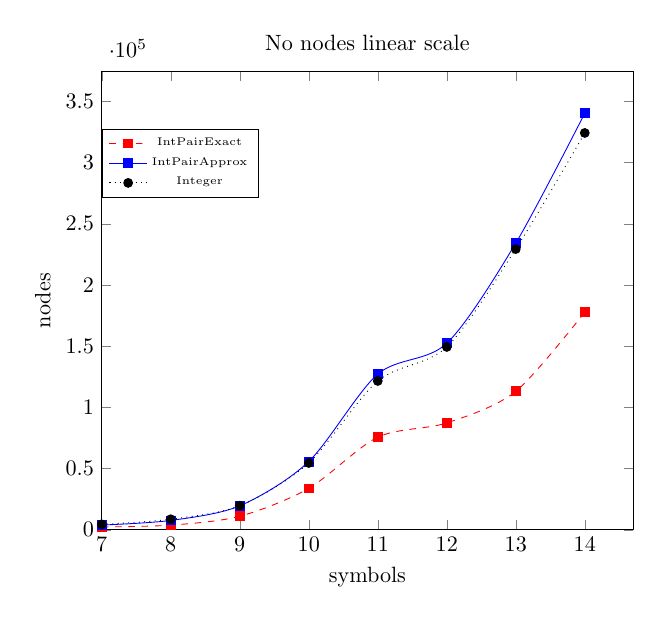
\begin{tikzpicture} [scale=0.8]
    \begin{axis}[
        title=No nodes linear scale,
        ylabel=nodes,
        xtick=data,
        ymin=0, 
        xlabel=symbols ]
      \addplot[smooth,mark=square*, mark options={solid},red, dashed]
      coordinates{ (7, 2397) (8, 3806) (9, 11079) (10, 33853) (11, 75698) (12, 87336) (13, 113148) (14, 177889)
      }; \label{ie_plot} \addlegendentry{IntPairExact}
      \addplot[smooth,mark=square*, mark options={solid},blue]
      coordinates{ (7, 3900) (8, 7665) (9, 19595) (10, 55807) (11, 127240) (12, 152406) (13, 234257) (14, 340410)
      }; \label{ia_plot} \addlegendentry{IntPairApprox}
      \addplot[smooth,mark=*,mark options={solid},black, dotted]
      coordinates{ (7, 4474) (8, 8637) (9, 19738) (10, 54608) (11, 121629) (12, 149424) (13, 229421) (14, 324263)
      }; \label{int_plot} \addlegendentry{Integer}
    \end{axis}
  \end{tikzpicture}
  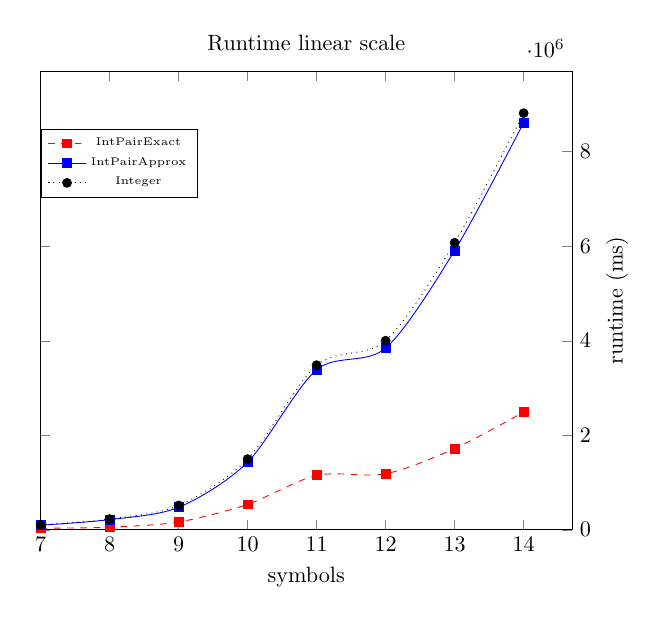
\begin{tikzpicture} [scale=0.8]
    \begin{axis}[
        yticklabel pos=right,
        xtick=data,
        title=Runtime linear scale,
        ylabel=runtime (ms),
        xlabel=symbols,
        ymin=0, ]
      \addplot[smooth,mark=square*,mark options={solid},red, dashed]
      coordinates{ (7,33465) (8,55016) (9,166184) (10,538149) (11,1151930) (12,1184668) (13,1718874) (14,2490040)
      }; \label{IntPairExact Run}
      \addplot[smooth,mark=square*,mark options={solid},blue]
      coordinates{ (7,97813) (8,215704) (9,475322) (10,1430987) (11,3386150) (12,3844124) (13,5907202) (14,8611872)
      }; \label{IntPairApprox Run}
      \addplot[smooth,mark=*,mark options={solid},black, dotted]
      coordinates{ (7,107122) (8,226900) (9,515144) (10,1495850) (11,3482780) (12,4001064) (13,6072058) (14,8813384)
      }; \label{IntegerRun}
      \addlegendentry{IntPairExact}
      \addlegendentry{IntPairApprox}
      \addlegendentry{Integer}
    \end{axis}
  \end{tikzpicture}

  
\begin{tikzpicture}[scale=1.4]
    \draw[very thick] (-4,0) -- (4,0);
    \draw[draw=white] (-5,-0.2) -- (5,-0.2);
  \end{tikzpicture}


  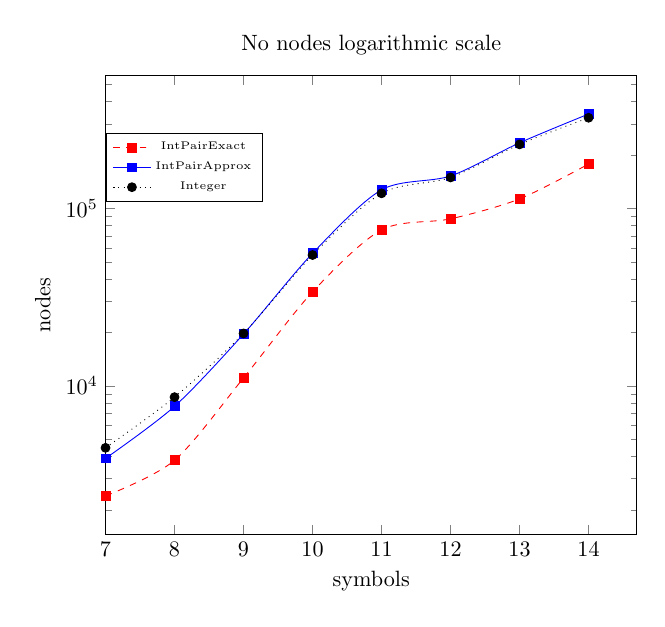
\begin{tikzpicture} [scale=0.8]
    \begin{semilogyaxis}[
        title=No nodes logarithmic scale,
        ylabel=nodes,
        xtick=data,
        ymin=0, 
        xlabel=symbols ]
     \addplot[smooth,mark=square*, mark options={solid},red, dashed]
      coordinates{ (7, 2397) (8, 3806) (9, 11079) (10, 33853) (11, 75698) (12, 87336) (13, 113148) (14, 177889)
      }; \label{ie_plot} \addlegendentry{IntPairExact}
      \addplot[smooth,mark=square*, mark options={solid},blue]
      coordinates{ (7, 3900) (8, 7665) (9, 19595) (10, 55807) (11, 127240) (12, 152406) (13, 234257) (14, 340410)
      }; \label{ia_plot} \addlegendentry{IntPairApprox}
      \addplot[smooth,mark=*,mark options={solid},black, dotted]
      coordinates{ (7, 4474) (8, 8637) (9, 19738) (10, 54608) (11, 121629) (12, 149424) (13, 229421) (14, 324263)
      }; \label{int_plot} \addlegendentry{Integer}

    \end{semilogyaxis}
  \end{tikzpicture}
  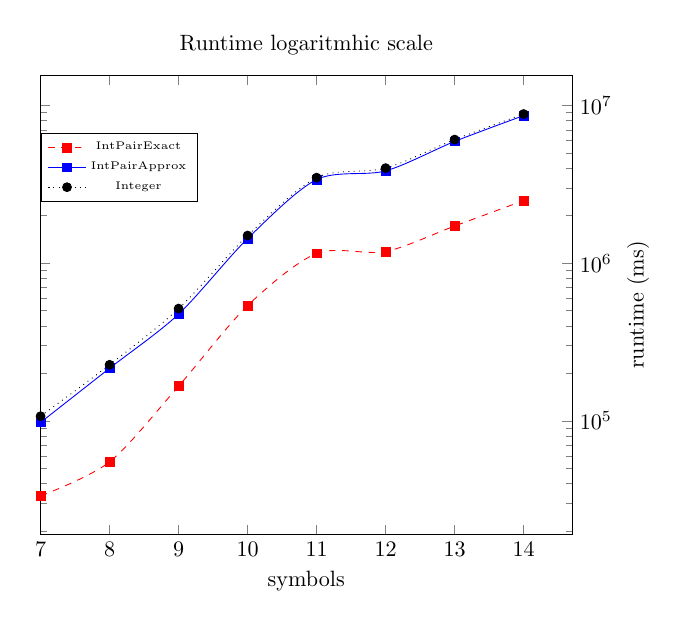
\begin{tikzpicture} [scale=0.8]
    \begin{semilogyaxis}[
        title=Runtime logaritmhic scale,
        yticklabel pos=right,
        xtick=data,
        ylabel=runtime (ms),
        xlabel=symbols,
        ymin=0,  ]
      \addplot[smooth,mark=square*,mark options={solid},red, dashed]
      coordinates{ (7,33465) (8,55016) (9,166184) (10,538149) (11,1151930) (12,1184668) (13,1718874) (14,2490040)
      }; \label{IntPairExact Run}
      \addplot[smooth,mark=square*,mark options={solid},blue]
      coordinates{ (7,97813) (8,215704) (9,475322) (10,1430987) (11,3386150) (12,3844124) (13,5907202) (14,8611872)
      }; \label{IntPairApprox Run}
      \addplot[smooth,mark=*,mark options={solid},black, dotted]
      coordinates{ (7,107122) (8,226900) (9,515144) (10,1495850) (11,3482780) (12,4001064) (13,6072058) (14,8813384)
      }; \label{IntegerRun}
      \addlegendentry{IntPairExact}
      \addlegendentry{IntPairApprox}
      \addlegendentry{Integer}
    \end{semilogyaxis}
  \end{tikzpicture}
  \caption{{Caption}}\label{fig:}
\end{figure}
